\section{Marco Teórico }
\subsection{Series de Fourier}

Las series de Fourier son una herramienta matemática que permite representar funciones periódicas como una suma de funciones sinusoidales. Cualquier función periódica continua puede ser representada por una serie de Fourier. Estas series surgen de la tarea práctica de representar una función periódica dada en términos de funciones coseno y seno. Estas series son trigonométricas cuyos coeficientes se determinan a partir de () mediante ciertas fórmulas (fórmulas de Euler), las cuales se establecerán primero. Después se considerará la teoría de las series de Fourier.

Las series de Fourier permiten identificar los componentes de frecuencia de una señal y su comportamiento a lo largo del tiempo por lo que la transformada de Fourier es una herramienta matemática que permite calcular los coeficientes de la serie de Fourier de una función.

La idea principal detrás de las series de Fourier es que cualquier señal periódica puede ser descompuesta en una suma infinita de componentes sinusoidales de diferentes frecuencias, conocidas como armónicos. Esta descomposición permite analizar y entender el comportamiento de la señal en términos de sus componentes básicos.

Matemáticamente, una serie de Fourier para una función periódica f(x) con período T se expresa como la \emph{serie de Fourier}\eqref{eq:serie_de_fourier}.
\begin{figure}[H]
	\begin{equation}
	\operatorname{f}(t) = \frac{a_0}{2} + \sum_{n=1}^{+\infty} (a_n \cos(nt) + b_n \sin(nt))	
	\label{eq:serie_de_fourier}
\end{equation}
\caption{Serie de Fourier}
\end{figure}


Donde posteriormente existe la participación de las fórmulas de Euler

\begin{figure}[H]
	\begin{equation}
		\begin{aligned}
			a_n &= \frac{1}{\pi} \int_{-\pi}^{\pi} \operatorname{f}(x) \cos(nt) \dd{t} \quad \text{para todo } n \geq 0 \\
			b_n &= \frac{1}{\pi} \int_{-\pi}^{\pi} \operatorname{f}(x) \sin(nt) \dd{t} \quad \text{para todo } n > 0
		\end{aligned}
		\label{eq:fourier_coeffs}
	\end{equation}
	\caption{Coeficientes de la Serie de Fourier}
\end{figure}

Finalmente los números dados en \eqref{eq:fourier_coeffs} se denominan coeficientes de Fourier de \(\operatorname{f}(t)\). La serie trigonométrica con coeficientes dados, \emph{a y b} se denomina serie de Fourier de \(\operatorname{f}(t)\).

La forma canónica de las series de Fourier es la que hemos estado utilizando hasta el momento, donde la función en cuestión estaba definida sobre el intervalo \([-\pi, \pi]\).

\subsection{Cómputo paralelo}

El cómputo paralelo es una técnica que permite ejecutar programas en varios procesadores al mismo tiempo.

Existen diferentes modelos de programación para el cómputo paralelo, como el modelo SPMD, el modelo MPI y el modelo OpenMP. La comunicación entre procesadores es un factor importante para el rendimiento del cómputo paralelo, además la escalabilidad es la capacidad de un programa para ejecutarse de manera eficiente en un número creciente de procesadores.

Hay muchas áreas de aplicación donde el poder de cálculo de una computadora simple es insuficiente para obtener los resultados deseados. Las computadoras paralelas y distribuidas pueden producir resultados más rápidos. Por ejemplo, en algunas áreas de cálculo científico, el tiempo estimado de computación para obtener resultados interesantes usando un computador simple, podría ser tan largo que excedería el tiempo esperado en que el mismo puede fallar.

La computación juega un papel fundamental en las ciencias y las ingenierías, permitiendo a los científicos e ingenieros construir y probar modelos con nuevas teorías para describir fenómenos naturales o para resolver problemas de la vida real. Estos modelos matemáticos altamente complejos son gobernados, por ejemplo, por ecuaciones diferenciales parciales o elementos finitos cuyas soluciones pueden requerir grandes poderes de cálculo. El modelado matemático consiste en describir entidades (estructuras complejas, procesos químicos o biológicos, etc.) en términos de ecuaciones que comprenden variables y constantes

Por ejemplo, las series de Fourier se pueden utilizar para descomponer un problema en una serie de subproblemas más pequeños que se pueden resolver en paralelo. Existen algoritmos paralelos para el cálculo de la transformada de Fourier y para la resolución de ecuaciones diferenciales que utilizan series de Fourier. El cómputo paralelo puede utilizarse para acelerar la ejecución de aplicaciones que utilizan series de Fourier.

Los computadores paralelos se han desarrollado estos últimos años gracias a los avances en campos tan diversos como el arquitectónico, las tecnologías de interconexión, los ambientes de programación (lenguajes, sistemas, etc.), como de otros más. Muchos esquemas de clasificación se han propuesto, pero el más popular es la taxonomía de Flynn, la idea central que se usa se basa en el análisis del flujo de instrucciones y de datos, los cuales pueden ser simples o múltiples, originando la aparición de 4 tipos de máquinas. Es decir, esta clasificación está basada en el número de flujos de instrucciones y de datos simultáneos. Según eso, las posibles categorías son:

\textbf{SISD (Single Instruction Stream, Single Data Stream)}

Esta representa la clásica máquina de Von-Neumann, en la cual un único programa es ejecutado usando solamente un conjunto de datos específicos a él.

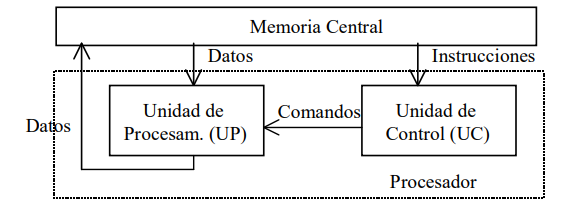
\includegraphics[width=3.18229in,height=1.17579in]{media/image38.png}

\emph{Imagen 3 - SISD}

\textbf{SIMD (Single Instruction Stream, Multiple Data Stream)}

Arreglo de elementos de procesamiento, todos los cuales ejecutan la misma instrucción al mismo tiempo.

El enfoque de paralelismo usado aquí se denomina paralelismo de datos. Los arreglos de procesadores son típicos ejemplos de esta clase de arquitectura. En estas arquitecturas, un controlador recibe y decodifica secuencias de instrucciones a ejecutar, para después enviarlas a múltiples procesadores esclavos.

Su funcionamiento es el siguiente: un simple controlador envía las instrucciones, una a una, a un arreglo de procesadores que operan en el esquema maestro-esclavo. Es decir, las instrucciones son difundidas desde la memoria a un conjunto de procesadores. Así, cada procesador es simplemente una unidad aritmética-lógica y se tiene una sola unidad de control. Todos los procesadores ejecutan cada operación recibida al mismo tiempo, por lo cual, cada uno ejecuta la misma instrucción sobre diferentes datos.

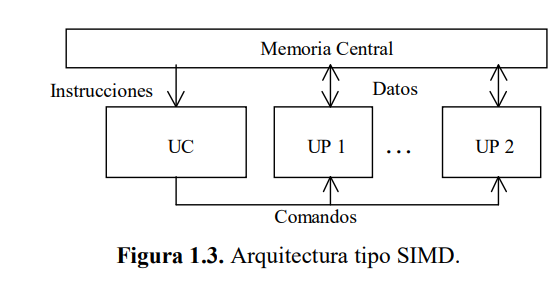
\includegraphics[width=3.19271in,height=1.43274in]{media/image33.png}

\emph{Imagen 4 - SIMD}
